\bigskip
\section{More in the online help}\label{sec:more}
These pages of the Help are summarised here. Scan a code, or click a title's link, to read the full page; it's also in the app under \textbf{Help}.\par\medskip

\begin{pagecard}\phantomsection\addcontentsline{toc}{subsection}{Set up exam questions}\label{sec:exam-questions}
{\large\bfseries Set up exam questions}\par\smallskip
The app reads the questions from the exam PDF (lines like \texttt{Q1. Using VMS109, \ldots{}}) or from an exam file. When that doesn't work, or gets something wrong, set the questions up yourself in the question editor.\par
\par\smallskip{\centering\tcbox[enhanced, boxsep=0pt, left=0pt, right=0pt, top=0pt, bottom=0pt, arc=4pt, boxrule=0.5pt, colframe=black, colback=white, clip upper]{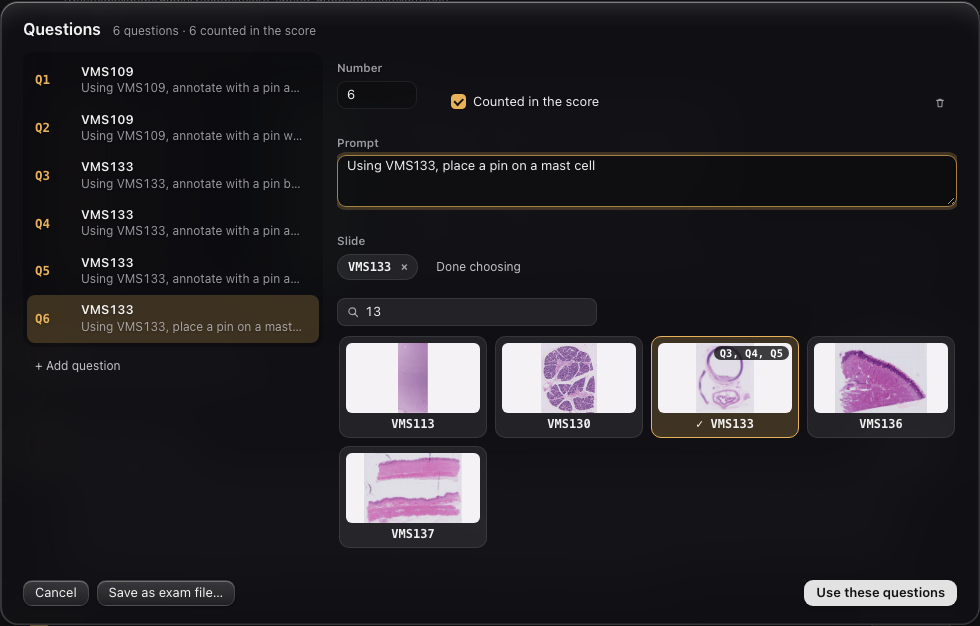
\includegraphics[width=0.7\linewidth, height=4.2cm, keepaspectratio]{img/exam-editor.png}}\par{\scriptsize The question editor}\par}\smallskip
{\small Covers: Before grading starts \textperiodcentered{} Choose slides \textperiodcentered{} Save as an exam file \textperiodcentered{} Inside a session}
\tcblower
\centering\href{https://github.com/agadin/micro-speed-grader/blob/main/docs/help/exam-questions.md}{\qrcode[height=1.75cm, nolink]{https://github.com/agadin/micro-speed-grader/blob/main/docs/help/exam-questions.md}}\\[3pt]\helplink{exam-questions.md}
\end{pagecard}

\begin{pagecard}\phantomsection\addcontentsline{toc}{subsection}{Clusters and navigation}\label{sec:clusters}
{\large\bfseries Clusters and navigation}\par\smallskip
Pins that land near each other are grouped into a \textbf{cluster}. Two settings in the right panel's \textbf{Clusters} section control it:\par

{\small Covers: How clusters work \textperiodcentered{} Moving around \textperiodcentered{} Images \textperiodcentered{} The minimap and scale \textperiodcentered{} Measure distances and areas}
\tcblower
\centering\href{https://github.com/agadin/micro-speed-grader/blob/main/docs/help/clusters.md}{\qrcode[height=1.75cm, nolink]{https://github.com/agadin/micro-speed-grader/blob/main/docs/help/clusters.md}}\\[3pt]\helplink{clusters.md}
\end{pagecard}

\begin{pagecard}\phantomsection\addcontentsline{toc}{subsection}{The ledger and undo}\label{sec:ledger}
{\large\bfseries The ledger and undo}\par\smallskip
The \textbf{Ledger} under the slide lists every grade on this image: one row per group of pins you graded together, with its reason and pin count. Tick \textbf{All images} to see the whole exam.\par
\par\smallskip{\centering\tcbox[enhanced, boxsep=0pt, left=0pt, right=0pt, top=0pt, bottom=0pt, arc=4pt, boxrule=0.5pt, colframe=black, colback=white, clip upper]{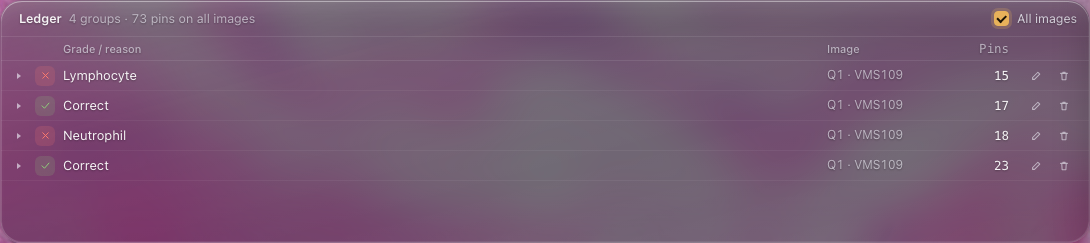
\includegraphics[width=0.7\linewidth, height=4.2cm, keepaspectratio]{img/ledger.png}}\par{\scriptsize The ledger}\par}\smallskip
{\small Covers: What you can do with a row \textperiodcentered{} Search and filter \textperiodcentered{} Undo and redo}
\tcblower
\centering\href{https://github.com/agadin/micro-speed-grader/blob/main/docs/help/ledger.md}{\qrcode[height=1.75cm, nolink]{https://github.com/agadin/micro-speed-grader/blob/main/docs/help/ledger.md}}\\[3pt]\helplink{ledger.md}
\end{pagecard}

\begin{pagecard}\phantomsection\addcontentsline{toc}{subsection}{Look up a student}\label{sec:students}
{\large\bfseries Look up a student}\par\smallskip
When a student asks about their grade, you don't need to hunt image by image. The student panel shows everything about one student: every question, what they answered, who graded it and why, and the feedback they'll get. You can check each pin on the slide and change a grade from there.\par
\par\smallskip{\centering\tcbox[enhanced, boxsep=0pt, left=0pt, right=0pt, top=0pt, bottom=0pt, arc=4pt, boxrule=0.5pt, colframe=black, colback=white, clip upper]{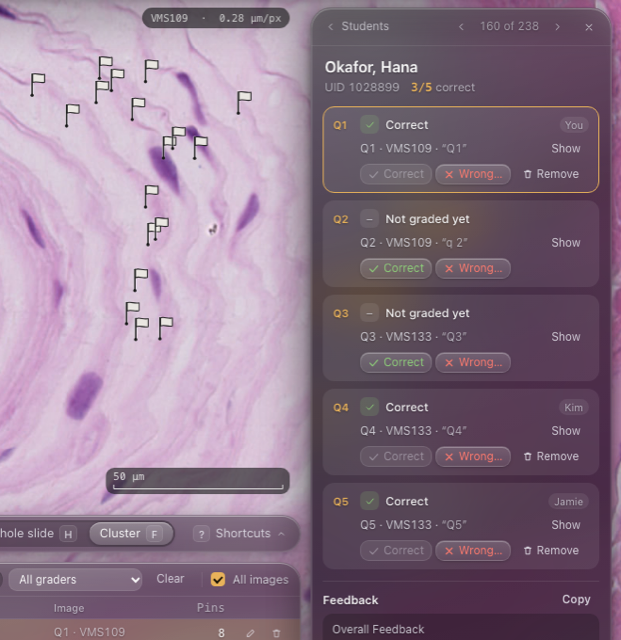
\includegraphics[width=0.7\linewidth, height=4.2cm, keepaspectratio]{img/students.png}}\par{\scriptsize The student panel beside the slide}\par}\smallskip
{\small Covers: Open a student \textperiodcentered{} What it shows \textperiodcentered{} Change a grade}
\tcblower
\centering\href{https://github.com/agadin/micro-speed-grader/blob/main/docs/help/students.md}{\qrcode[height=1.75cm, nolink]{https://github.com/agadin/micro-speed-grader/blob/main/docs/help/students.md}}\\[3pt]\helplink{students.md}
\end{pagecard}

\begin{pagecard}\phantomsection\addcontentsline{toc}{subsection}{What students see}\label{sec:feedback}
{\large\bfseries What students see}\par\smallskip
Every student gets a short feedback note built from your grades. The same text goes into their own \texttt{feedback/\textless{}name\textgreater{}.txt} file and into the \textbf{Comment} column of \texttt{grades.csv}.\par
\par\smallskip{\centering\tcbox[enhanced, boxsep=0pt, left=0pt, right=0pt, top=0pt, bottom=0pt, arc=4pt, boxrule=0.5pt, colframe=black, colback=white, clip upper]{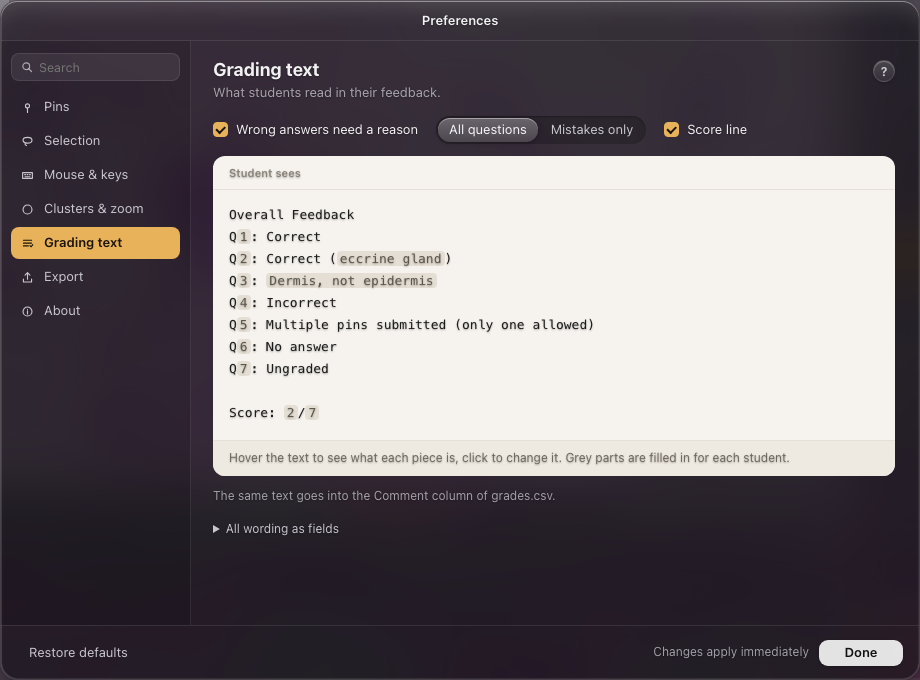
\includegraphics[width=0.7\linewidth, height=4.2cm, keepaspectratio]{img/prefs-text.png}}\par{\scriptsize Editing the feedback wording}\par}\smallskip
{\small Covers: Changing the wording}
\tcblower
\centering\href{https://github.com/agadin/micro-speed-grader/blob/main/docs/help/feedback.md}{\qrcode[height=1.75cm, nolink]{https://github.com/agadin/micro-speed-grader/blob/main/docs/help/feedback.md}}\\[3pt]\helplink{feedback.md}
\end{pagecard}

\begin{pagecard}\phantomsection\addcontentsline{toc}{subsection}{Preferences}\label{sec:preferences}
{\large\bfseries Preferences}\par\smallskip
Open Preferences with \keycap{\cmdsym{}}\keyplus{}\keycap{,} or the gear in the top bar. It opens in its own window; changes apply immediately. Type in the search field at the top of the sidebar to find a setting. \textbf{Restore defaults} resets everything.\par

{\small Covers: Pins \textperiodcentered{} Selection \textperiodcentered{} Mouse \& keys \textperiodcentered{} Clusters \& zoom \textperiodcentered{} Reading submissions \textperiodcentered{} Grading text \textperiodcentered{} Export \textperiodcentered{} About}
\tcblower
\centering\href{https://github.com/agadin/micro-speed-grader/blob/main/docs/help/preferences.md}{\qrcode[height=1.75cm, nolink]{https://github.com/agadin/micro-speed-grader/blob/main/docs/help/preferences.md}}\\[3pt]\helplink{preferences.md}
\end{pagecard}

\begin{pagecard}\phantomsection\addcontentsline{toc}{subsection}{Troubleshooting}\label{sec:troubleshooting}
{\large\bfseries Troubleshooting}\par\smallskip
\textbf{"No questions like ``Q1. Using VMS123, \ldots{}'' were found in that file."} The exam's questions must start like \texttt{Q1. Using VMS109, \ldots{}}. If the PDF is a scan (an image with no text), make a JSON exam file instead:\par

{\small Covers: Setting up a session \textperiodcentered{} While grading \textperiodcentered{} Updates \textperiodcentered{} Still stuck?}
\tcblower
\centering\href{https://github.com/agadin/micro-speed-grader/blob/main/docs/help/troubleshooting.md}{\qrcode[height=1.75cm, nolink]{https://github.com/agadin/micro-speed-grader/blob/main/docs/help/troubleshooting.md}}\\[3pt]\helplink{troubleshooting.md}
\end{pagecard}
